\documentclass[8pt]{beamer}\usepackage[]{graphicx}\usepackage[]{xcolor}
% maxwidth is the original width if it is less than linewidth
% otherwise use linewidth (to make sure the graphics do not exceed the margin)
\makeatletter
\def\maxwidth{ %
  \ifdim\Gin@nat@width>\linewidth
    \linewidth
  \else
    \Gin@nat@width
  \fi
}
\makeatother

\definecolor{fgcolor}{rgb}{0.345, 0.345, 0.345}
\newcommand{\hlnum}[1]{\textcolor[rgb]{0.686,0.059,0.569}{#1}}%
\newcommand{\hlstr}[1]{\textcolor[rgb]{0.192,0.494,0.8}{#1}}%
\newcommand{\hlcom}[1]{\textcolor[rgb]{0.678,0.584,0.686}{\textit{#1}}}%
\newcommand{\hlopt}[1]{\textcolor[rgb]{0,0,0}{#1}}%
\newcommand{\hlstd}[1]{\textcolor[rgb]{0.345,0.345,0.345}{#1}}%
\newcommand{\hlkwa}[1]{\textcolor[rgb]{0.161,0.373,0.58}{\textbf{#1}}}%
\newcommand{\hlkwb}[1]{\textcolor[rgb]{0.69,0.353,0.396}{#1}}%
\newcommand{\hlkwc}[1]{\textcolor[rgb]{0.333,0.667,0.333}{#1}}%
\newcommand{\hlkwd}[1]{\textcolor[rgb]{0.737,0.353,0.396}{\textbf{#1}}}%
\let\hlipl\hlkwb

\usepackage{framed}
\makeatletter
\newenvironment{kframe}{%
 \def\at@end@of@kframe{}%
 \ifinner\ifhmode%
  \def\at@end@of@kframe{\end{minipage}}%
  \begin{minipage}{\columnwidth}%
 \fi\fi%
 \def\FrameCommand##1{\hskip\@totalleftmargin \hskip-\fboxsep
 \colorbox{shadecolor}{##1}\hskip-\fboxsep
     % There is no \\@totalrightmargin, so:
     \hskip-\linewidth \hskip-\@totalleftmargin \hskip\columnwidth}%
 \MakeFramed {\advance\hsize-\width
   \@totalleftmargin\z@ \linewidth\hsize
   \@setminipage}}%
 {\par\unskip\endMakeFramed%
 \at@end@of@kframe}
\makeatother

\definecolor{shadecolor}{rgb}{.97, .97, .97}
\definecolor{messagecolor}{rgb}{0, 0, 0}
\definecolor{warningcolor}{rgb}{1, 0, 1}
\definecolor{errorcolor}{rgb}{1, 0, 0}
\newenvironment{knitrout}{}{} % an empty environment to be redefined in TeX

\usepackage{alltt}

\usepackage[french]{babel}
\usepackage[utf8]{inputenc}%pour que latex comprenne les accents
\usepackage[T1]{fontenc}%pour que latex imprime les accents
\usepackage{multicol}%pour créer plusieurs colonnes
\usepackage{amsmath}
\usepackage{graphicx}


\usetheme{CambridgeUS}%thème que l'on peut changer si l'on veut
\usepackage{pdfpages}
%

% mise en forme des paragraphes
\usepackage{parskip}% saut de lignes en fin de paragraphe
\let\EndItemize\enditemize
\def\enditemize{\EndItemize\bigskip}% sauts de ligne en fin d'environnement itemize

% tables et figures
\usepackage{multirow} % permet de fusionner les colonnes
\usepackage{graphicx} % admet les figures
\usepackage{array} % types particuliers de tableaux
\usepackage{tabularx} % autres tableaux, notamment pour gérer les doubles traits de séparation (voir hhline)
\usepackage[hang,small]{caption} % mise en forme du caption

% lignes de code
\usepackage{minted}
\usepackage{listings}  % pour les chunk
\setminted{breaklines} % pour sauter des lignes
\definecolor{bg}{rgb}{0.95,0.95,0.95}

% page de titre
\title{Petite introduction à \LaTeX{} en Sciences Sociales}
\author{Julio Ricardo Davalos}
\institute{CEMS (EHESS-Inserm)}
\makeatletter
\setbeamercolor{autre}{fg = black, bg = white}
\setbeamercolor{title}{fg = red, bg = white}
\setbeamertemplate{title page}%pour changer la mise en forme de la page de titre
{
  \begin{centering}
    \begin{beamercolorbox}[sep=8pt,center, rounded = true, shadow = true]{title}%titre
      \Huge\inserttitle\par%
      \ifx\insertsubtitle\@empty%
      \else%
        \vskip0.25em%
        {\usebeamerfont{subtitle}\usebeamercolor[fg]{subtitle}\insertsubtitle\par}%
      \fi%     
    \end{beamercolorbox}
    \begin{beamercolorbox}[sep=8pt,center,]{autre}%le reste
        \Large\insertauthor\\
        \large\insertinstitute\\
        \large\insertdate
    \end{beamercolorbox}%\vskip0.5em
  \end{centering}
}

\newcommand{\nomfonction}[2][]{\texttt{\textbackslash#2\{#1\}}}
\IfFileExists{upquote.sty}{\usepackage{upquote}}{}
\begin{document}
	\begin{frame}
    \titlepage
	\end{frame}
	
		\begin{frame}
	  \begin{block}{C'est quoi \LaTeX?}
	    \begin{itemize}
	      \item un système de composition de document qui permet de produire une mise en page propre et automatisée
	      \item utilisé généralement dans un éditeur de texte pouvant compiler du code (\TeX maker)
	      \item[$\neq$] traitement de texte qui doit donc en permanence rafraîchir la mise en forme du texte
	      \item[$\Rightarrow$] Séparation du fond et de la forme
	    \end{itemize}
	  \end{block}
	  \begin{alertblock}{Mais quel est l'intérêt de l'utilisation de \LaTeX?}
	    \begin{itemize}
	    \item le plus connu: les mathématiques
	      \begin{equation}
  f(x)=\frac{\sqrt{x}}{x} % racine carrée
  \end{equation}
	    \item une mise en page harmonieuse
	    \item Pas d'affichage en temps réel $=$ gain de performance
	    \item[$\Rightarrow$] et donc gain en qualité typographique pour moins de temps cumulé de calcul
	    \item[$\Rightarrow$] possibilité de faire de gros fichiers sans bug
	    \item automatisation de la mise en page (appel d'un package ou ajout d'une caractéristique)
	    \item idem sur la bibliographie, l'index, la table des matières etc.
	    \item[$\Rightarrow$] gain de temps sur la forme 
	    \end{itemize}
	  \end{alertblock}
	\end{frame}
	\begin{frame}
	\begin{figure}[h!]
  \caption{Schéma de la marge de progression entre \LaTeX{} et Word}
  \label{exemple_ref}
  \centering
  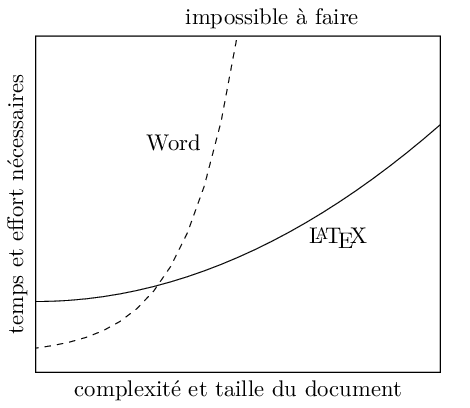
\includegraphics[scale=0.5]{Images/latex_word.png}
\end{figure}
	\end{frame}
	\begin{frame}
    \tableofcontents
	\end{frame}


\section{Les principes de base de \LaTeX}
\subsection{Installation}

	\begin{frame}{Installation}
\begin{block}{Windows}
	    \begin{itemize}
	      \item Mik\TeX{} ou \TeX Live
	      \item \TeX Live a tendance a avoir moins d'erreurs dans mon expérience mais plus compliqué à installer
	    \end{itemize}
	  \end{block}
	  
\begin{block}{MacOS}
	    \begin{itemize}
	      \item uniquement \TeX Live
	      \item[$\Rightarrow$] très simple à installer!
	    \end{itemize}
	  \end{block}
	  
   \begin{block}{Linux}
    \texttt{sudo apt-get install texlive-full}
	  \end{block}
	\end{frame}


\subsection{Fonctionnement de la compilation}
	\begin{frame}{Compilation}
	\begin{figure}[h!]
  \caption{Schéma explicatif de la compilation}
  \label{compilation}
  \centering
  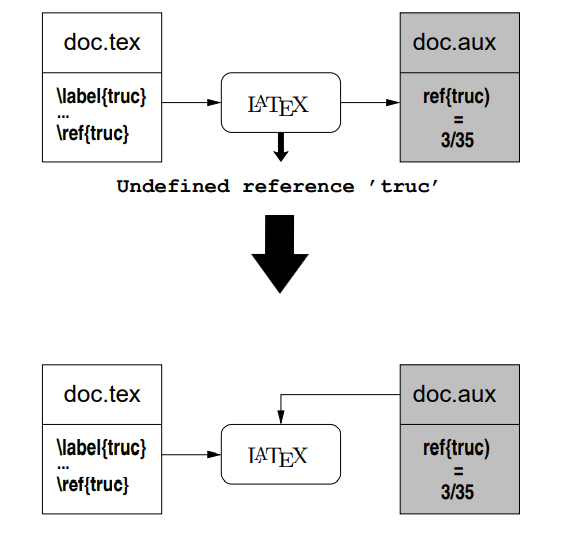
\includegraphics[scale=0.4]{Images/compilation.png}
\end{figure}
	\end{frame}

\subsection{Notions principales}
	\begin{frame}{Notions principales}
	 \begin{block}{Package}
	  \begin{itemize}
    \item comme dans R
    \item la documentation est très fournie et les forums aussi
    \item à charger en début de document
    \end{itemize}
	  \end{block}
	  
	 \begin{block}{Préambule}
	\begin{figure}[h!]
  \caption{Structure du code \LaTeX}
  \label{preambule}
  \centering
  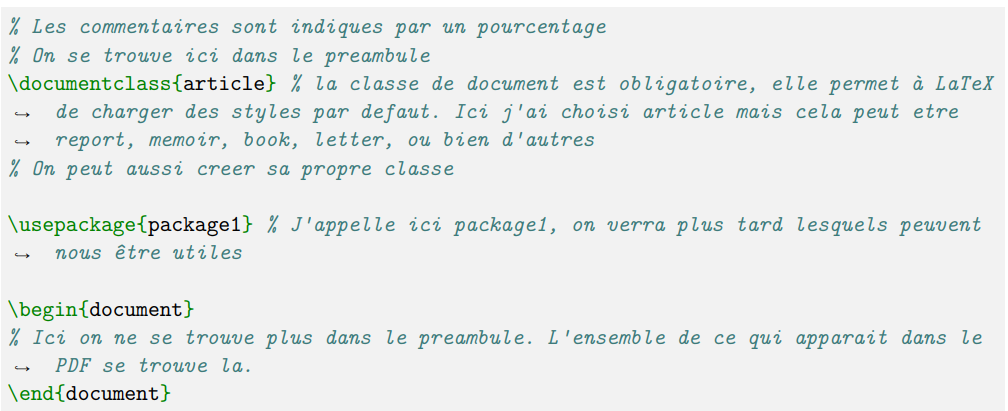
\includegraphics[scale=0.36]{Images/preambule.png}
\end{figure}
	  \end{block}
	 
	\end{frame}
	
	\begin{frame}{Notions principales}
	 \begin{block}{Environnement}
	 \begin{itemize}
 \item espace délimité dans lequel certaines règles précises et certaines fonctions ont cours
 \item \texttt{document} est un environnement, \texttt{equation} aussi etc
 \begin{figure}
 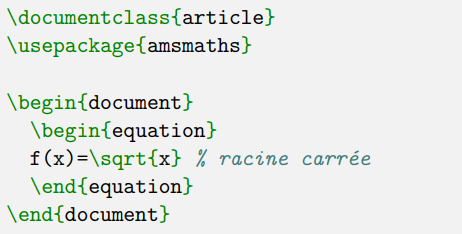
\includegraphics[scale=0.36]{Images/equation.png}
 \end{figure}
\end{itemize}
\begin{equation}
  f(x)=\sqrt{x} % racine carrée
  \end{equation}
	  \end{block}
	  
	 \begin{block}{Classe de document}
	 $\Rightarrow$ article, report, book, memoir
	  \begin{table}[!ht]
  \centering\footnotesize
  \begin{tabular}{|l|l|c|}
  \hline Commande & Sens & Niveau\\
  \hline \nomfonction{part} & Partie & $-1$\\
  \nomfonction{chapter} & Chapitre & $0$\\
  \nomfonction{section} & Section & $1$\\
  \nomfonction{subsection} & Sous-section & $2$\\
  \nomfonction{subsubsection} & Sous-sous-section & $3$\\
  \nomfonction{paragraph} & Paragraphe & $4$\\
  \nomfonction{subparagraph} & Sous-paragraphe & $5$\\
  \hline
  \end{tabular}
\end{table}
	  \end{block}
	\end{frame}
	
	\begin{frame}
	Des questions avant la partie pratique?
	\end{frame}

\section{Construction d'un document \LaTeX}
\subsection{Choix courants dans le préambule}
\subsection{Environnements et packages usuels}
\subsection{Corps du texte}
\subsection{Bibliographie}

\section{Mise en forme de résultats statistiques avec \LaTeX}
\subsection{Logique de RSweave}
\subsection{Exemples de tableaux}
\subsection{Exemple de figure}
	
	\begin{frame}
	\end{frame}



\end{document}
